
\graphicspath{ {mainmatter/Palacio-Quintin_2008/} }

\title*{2008: Eight Years of Practice on the Hyper-Flute: Technological and Musical Perspectives}
\titlerunning{Eight Years of Practice on the Hyper-Flute}
\author{Cl\'{e}o Palacio-Quintin}
\authorrunning{Palacio-Quintin}

\maketitle

\abstract*{After eight years of practice on the first hyper-flute prototype (a flute extended with sensors), this article presents a retrospective of its instrumental practice and the new developments planned from both technological and musical perspectives. Design, performance skills, and mapping strategies are discussed, as well as interactive composition and improvisation. }

\section{Introduction}

Since 1999, I have been performing on the hyper-flute~ \cite{Palacio-Quintin:2003}. Interfaced to a computer by means of electronic sensors and Max-MSP software, the extended flute enables me to directly control the digital processing parameters as they affect the flute's sound while performing and allows me to compose unusual electroacoustic soundscapes.

Until now, I mostly used the hyper-flute to perform improvised music.  Wishing to expand a repertoire for the hyper-flute, I began doctoral studies in January 2007 to work on written compositions. Before developing a core repertoire, I decided to review my experience with the instrument. 

This article presents the original design of the hyper-flute and the learning experience of eight years of practice on it. The performance skills and mapping strategies developed over time now suggest new enhancements of the instrument. Technological and musical issues in the development of a new prototype of the hyper-flute as well as a hyper-bass-flute will be discussed.

% FIGURE 1 - PHOTO 
%[bb=0 0 1080 810]

\begin{figure}[t]
\centering
	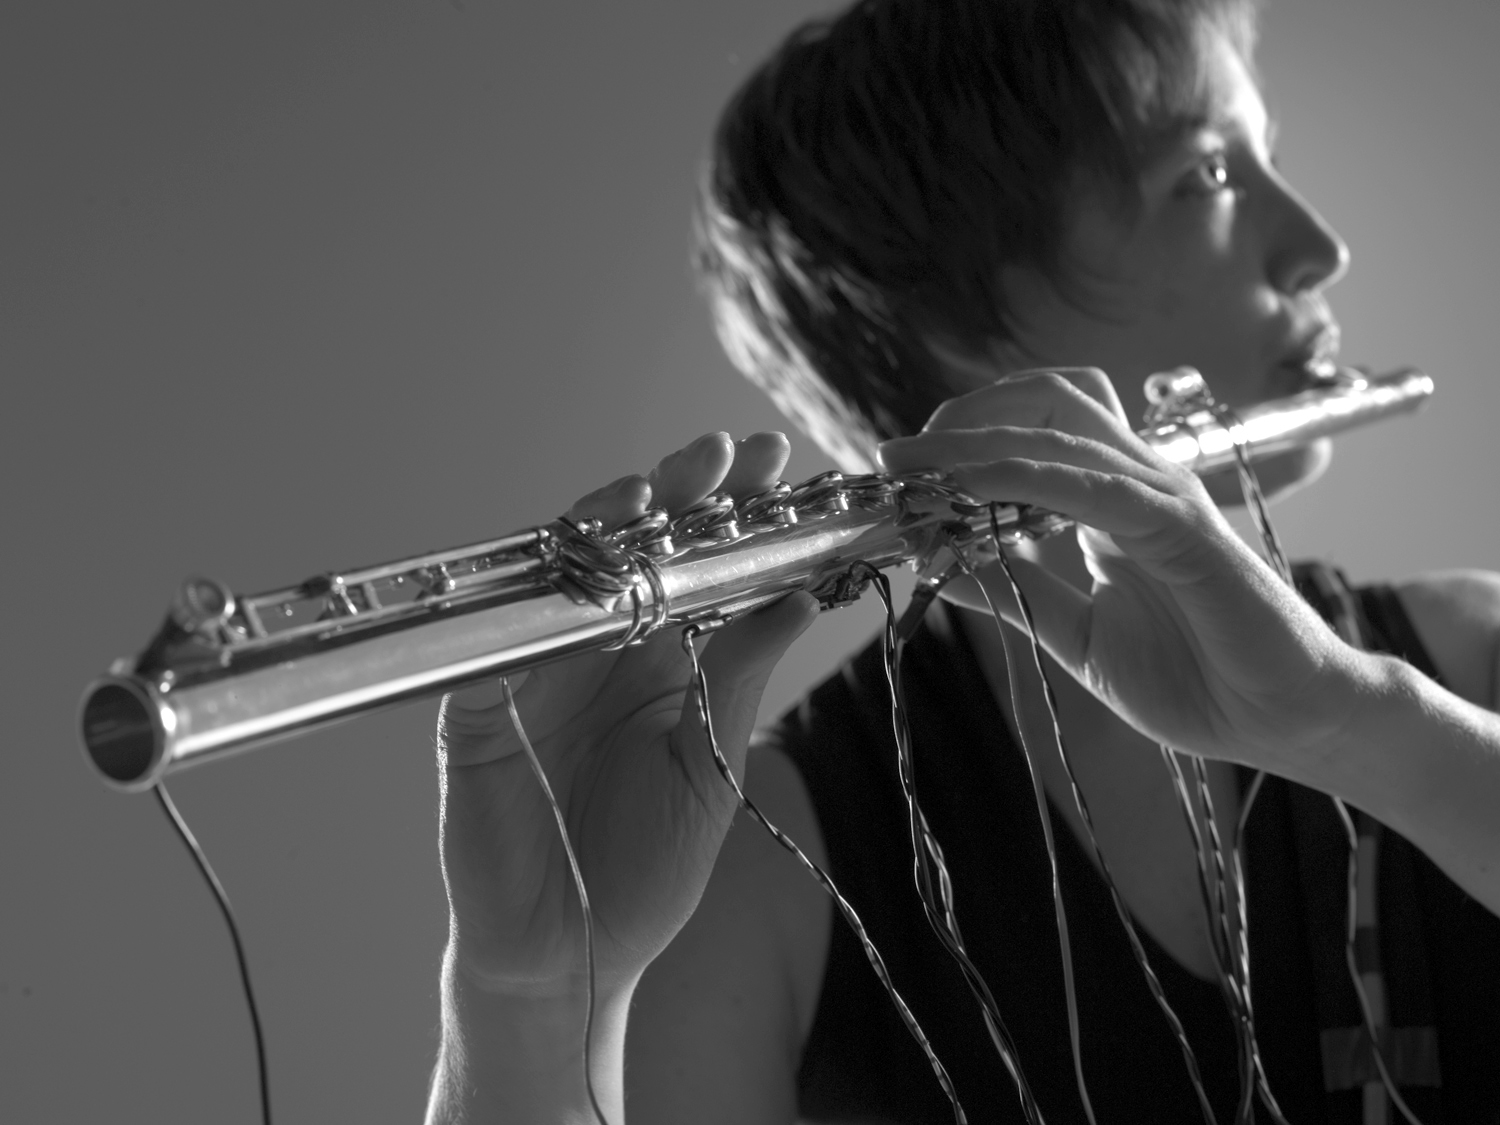
\includegraphics[width=\columnwidth]{CleoPQ-portrait.jpg}
\caption{The hyper-flute played by Cl\'{e}o Palacio-Quintin. Photograph by Carl Valiquet.}			
\label{Palacio-Quintin:photo}
\end{figure}


\section{Background}

\subsection{Why, Where and When} 

By the end of my studies in contemporary flute performance (Universit\'{e} de Montr\'{e}al, 1997), I was heavily involved in improvised music and had started looking for new sonorities for the flute in my own compositions.  Already familiar with electroacoustic music and with the use of the computer, it was an obvious step to get into playing flute with live electronics. My goal was to keep the acoustic richness of the flute and my way of playing it.  The computer would then become a virtual extension of the instrument. 

During post-graduate studies in Amsterdam, I had the chance to meet the experienced instrument designer Bert Bongers~ \cite{Bongers:2000}.  In 1999, I participated in the \textit{Interactive Electronic Music Composition/Performance course} with him and the  \textit{meta-trumpeter} Jonathan Impett~ \cite{Impett:1994} at the Dartington International Summer School of Music (U.K.). There, I made my first attempt at putting several sensors on my flute, programming a Max interface, and performing music with it.  Several months later, I registered as a student at the Institute of Sonology in The Hague (The Netherlands) in order to build my hyper-flute. The prototype of the hyper-flute was mainly built during the Fall of 1999 with the help of Lex van den Broek. Bert Bongers was a valuable consultant for the design. He also made the main connector from the sensors to the Microlab interface.

\subsection{Original Design} 

\subsubsection{Interface}
The Microlab is an electronic interface that converts the voltage variations from various analog sensors (between 0 and 5 volts) into standard MIDI data.  It offers 32 analog inputs, a keyboard matrix of 16 keys and an integrated ultrasonic distance measuring device. This interface was originally designed and developed by J. Scherpenisse and A.J. van den Broek at the Institute of Sonology. As a student there, I had access to the schematics and was able to build it myself.

\subsubsection{Sensors}

There is little free space to put hardware on a flute because of the complexity and small size of its key mechanism. Nevertheless it was possible to install sensors at specific strategic locations. Table~\ref{Palacio-Quintin:sensors-table} shows an overview of all the sensors installed on the hyper-flute.

% TABLE 1 - sensors

\begin{table}[t]
\label{Palacio-Quintin:sensors-table}
\centering
\ra{1.2}
\caption{Sensors installed on the hyper-flute}
\vspace{3pt} \noindent
\begin{tabular}{ll}
\toprule
\textbf{Sensors}     & \textbf{Parameter}  \\
\midrule  
1 Ultrasound sensors & flute's distance to computer\\
3 Pressure sensors (FSRs) & pressure: left hand and thumbs\\
2 Magnetic field sensors &  motion of G\# and low C\# keys\\
1 Light-dependent resistor & ambient light\\
2 Mercury tilt switches & tilt and rotation of the flute \\
6 Button switches & discrete cues \\
\bottomrule
\end{tabular}
\end{table}

Inspired by Jonathan Impett's meta-trumpet, I chose to put different types of electronic sensors on my flute. 

\begin{quotation}
As far as possible, this is implemented without compromising the richness of the instrument and its technique, or adding extraneous techniques for the performer---most of the actions already form part of conventional performance. \cite[p.148]{Impett:1994} 
\end{quotation}

The most important energy captors are proprioceptive sensors. These directly relate to instrumental playing. A performer is always aware of the action of her muscles on the instrument and her physical position. Of course a well trained musician is not really concious of these parameters while performing. They become unconscious gestures though always under her control. To collect gestural data, a number of proprioceptive sensors have been installed on the flute. 

Several analog sensors send continuous voltage variations to the Microlab which converts them into MIDI Continuous Controller messages.  Ultrasound transducers are used to track the distance of the flute from the computer.  An ultrasonic pulsed signal is sent by a transmitter attached to the computer, and is captured by the receiver attached to the flute's footjoint.  The Microlab calculates the distance based on the speed of sound.  Pressure sensors (Force Sensing Resistors) are installed on the principal holding points of the flute (under the left hand and the two thumbs). Two magnetic field sensors (Hall Effect) give the exact position of the G\# and low C\# keys, both operated by the little fingers. A light dependent resistor is positionned on the headjoint of the flute. This photoresistor detects the variations of ambient light. 

Other controllers used on the hyper-flute send discrete values : on/off Midi Note messages. Two mercury tilt switches are activated by the inclination (moving the footjoint up) and the rotation (turning the headjoint outwards) of the instrument. There are also six little button switches which can also be considered pressure sensors, but which send two discrete values (on/off) instead of continuous mesurements. Two of them are located on the headjoint, and two are placed close to each of the thumbs and can be reached while playing. 


\section{Learning Experience}

When I built the hyper-flute, I had  little knowledge about augmented instruments, and hardly any experience with human-computer interaction. Several choices of design were thus made because of technical considerations. Some of these choices were arbitrary and made without overt musical considerations. However, most decisions turned out to be quite pertinent. I will discuss design details and the use of sensors in relationship with the physicality of flute playing. Finally, I will present some of my ideas on performance skills and mapping strategies developed over the years. 


\subsection{Design \& Sensors}

When designing the hyper-flute some sensors were chosen simply because they were available. I just had to find a place to put them on the flute. This was the case for the ultrasound transducer and the light sensor. I also studied the free space available on the instrument and looked for what sort of sensor I could put there.  Since the G\# and low C\# keys are the only levers on the flute with space available under them, I installed the magnet sensors in those two places.
 
Because it does not compromise the natural movements of the fingers and hands for instrumental playing, the ultrasonic range finder integrated into the Microlab interface turned out to be one of the most useful controllers.  The same benefits comes from the tilt switches which are activated without any interaction of the fingers. 

As there is no movement involved, pressure sensors (FSR) are considered isometric. These sensors only capture muscle tension. This made it easier to get used to performing with them. A large FSR is installed under the left hand, which holds the flute by pressing it towards the chin. There is a constant contact and a continual variation of pressure on this point of the instrument while playing, though the pressure is quite controllable. 

Under the left thumb, a small FSR is placed on the B key. As this key is used to play, it moves often and is sometimes completely released. This limits the control of the sensor. A third FSR is located under the right thumb holding the flute. There is a constant variation of the pressure on the three sensors depending on what fingering is being played and how the instrument's balance is kept (for example: if a thumb if lifted, the two other holding points will get more of the weight of the instrument). These pressure sensors cannot be controlled without interacting with the playing but they do not interfere with the normal motion of the fingers and hands. They capture natural gestures related to the musical content performed. 

The pressure sensors also interact directly with the button switches. Four of them are located close to the thumbs and can be reached while playing. The respective thumb's pressure sensor is thus released when a button is used. The left thumb cannot reach buttons without compromising the fingering, while the right thumb is freer. Like the two mercury tilt switches, those buttons turned out to be very practical, even essential, to activate/desactivate various computer processes and to scroll through menus during performances. Two extra button switches, not easily reachable while playing, are located next to the headjoint. In order to perform without touching the computer, those switches are often used to start and end a piece. 
 
The magnet sensors give the exact position of the lever of the G\# and low C\# keys. The small distance of the action of the key is precisely mesured in 95 steps. It is possible to play with the motion range of the keys and make different curves for the midi output with quite accurate control. This is not a standard technique on the flute and it  affects the acoustics of the instrument.
 
Because it happened to be around at the time, a light sensor was installed on the instrument. I expected to use it with stage lighting.  However, staging with a lighting rig is quite uncommun when performing improvised electronic music. I have used it only once in 8 years. Realistically, I cannot control the ambient light myself, so this sensor is not really relevant.

Over the years, the entire design of the hyper-flute proved to be quite robust. Everything still works as well as on the first day. The force sensing resistors need to be replaced (more or less every 2 years) but all the other parts are still the original ones.  The Microlab interface is also very stable and reliable. Even as the MIDI protocol is becoming obsolete and slow compared to new standards, the stability of the interface has been a good help in developing performance skills for the long term.

\subsection{Performance Skills}

The detailed physical control required to perform on traditional acoustic instruments takes time to learn. I spent more than 15 years developing my instrumental skills. While playing an acoustic instrument, all performers receive mechanical feedback cues via a variety of physiological and perceptual signals. Haptic sensations include tactile and kinaesthetic perception. Kinaesthetic perception is the awareness of the body state, including position, velocity and forces supplied by the muscles. The auditory feedback is obviously very important but the physical sensation of playing comes before the perception of the sound. 

While extending my flute sound with computer processing, I wanted to keep the same subtle control. It was obvious that I should use my already refined instrumental skills in order to control the sound processing parameters. However, in order to perform proficiently on the hyper-flute, many extra techniques needed to be developed.

Earlier I mentioned that the ultrasonic device and the tilt switches were very useful because they do not compromise natural movements. However, the movements they capture are not normally necessary for flute playing. The performer is not trained to consciously notice them.  But once these sensors were linked to sound processing parameters, it was very difficult not to activate something without meaning to.  I had to learn to play completely motionless (which is very unnatural for a performer) in order to attain the necessary control.

In the case of the pressure sensors, they always react according to the fingerings played. It is almost impossible to keep them completely stable, but they are very flexible and the motion of pressing them is natural.  The maximum values are reachable only with extreme pressure which does not occur in normal playing although it can be used expressively. The process of learning to use those sensors has not been too difficult, as they are normal playing gestures simply needing, at times, to be exaggerated.

The control of the little fingers' magnetic sensors was much more difficult to learn. Flutists are trained to push or lift a key very fast as opposed to moving it slowly within its motion range. After hours of practice, I trained my little fingers and can now control those sensors quite accurately. 

Performing with some of the sensors installed on the hyper-flute was not always compatible with standard flute technique and entailed a long learning process. Playing an extended instrument requires a new way of performing.  This should be kept in mind by designers of new interfaces.  Few performers are willing to put a large amount of energy and time into learning to perform on a new instrument.

Experience showed me how much the interaction between acoustic playing techniques and the motion captured by the sensors is intimately connected. Musical gestures need to be thought of as a whole. You cannot simply ask a flutist to play normally and add extra motions to be captured by the sensors. All gestures need to be integrated in order to achieve expressive performances. 

Just like learning an acoustic instrument, it is necessary to play on an electroacoustic instrument for a long period of time before achieving a natural control of the sound. As on any musical instrument, expressivity is directly linked to virtuosity~ \cite{Dobrian:2006}. But in order for this to happen on the electroacoustic instrument, the mappings of gesture to sound must also remain stable.


\subsection{Mapping Strategies}

My first attempts at controlling sound processing parameters with the hyper-flute were made by directly coupling each sensor to a specific parameter of sound processing. This simple \emph{direct mapping} approach was soon changed. It is almost impossible for a performer to think about many different parameters, each controlled separately but simultaneously. It implies an analytical cognitive mode of thinking which is confusing for human beings while performing a complex task. Thinking in sequential order is very hard for a player who is already busy playing an acoustic instrument. 

Axel Mulder came to the same conclusion using a bodysuit with sensors, and trying to map each joint of the body to control a single synthesis parameter. 

\begin{quotation}
This mapping appeared to be very difficult to learn. First of all, human movements often involve the simultaneous movement of multiple limbs. So, when the intent was to change one or more specific parameter(s), often other synthesis parameters were co-articulated, i.e. also changed unintentionnaly. \cite[p.325]{Mulder:2000}
\end{quotation}


Researchers Hunt and Kirk have done experimental work to compare different types of interface mapping for real-time musical control tasks. This research revealed that  \emph{``complex tasks may need complex interfaces''} \cite[p.254]{Hunt:2000}, so the use of a multiparametric interface seems to be the best choice on the long-term in order to develop an interesting interactive system. The holistic mode of thinking involves looking at a perceived object as a whole. It relates to spatial thinking and is much more appropriate for multi-dimensional gestural control. 

An acoustic instrument is played in such a multiparametric way. 

\begin{quotation}
The resulting mapping of input parameters to sound parameters in a traditional acoustic instrument resembles a web of interconnections. \cite[p.235]{Hunt:2000} 
\end{quotation}

As illustrated in Figure~\ref{Palacio-Quintin:mapping}, the air pressure blown into a flute, which contributes to the pitch, also has an effect on the amplitude and timbre of the sound. The pitch is also affected by other inputs (fingerings, lip position). Each parameter of the sound is affected by different inputs simultaneously. 

% FIGURE 2 Example of multiparametric mapping of inputs to control flute sound 
%% bb=0 0 595 340
\begin{figure}
\centerline{\framebox{
	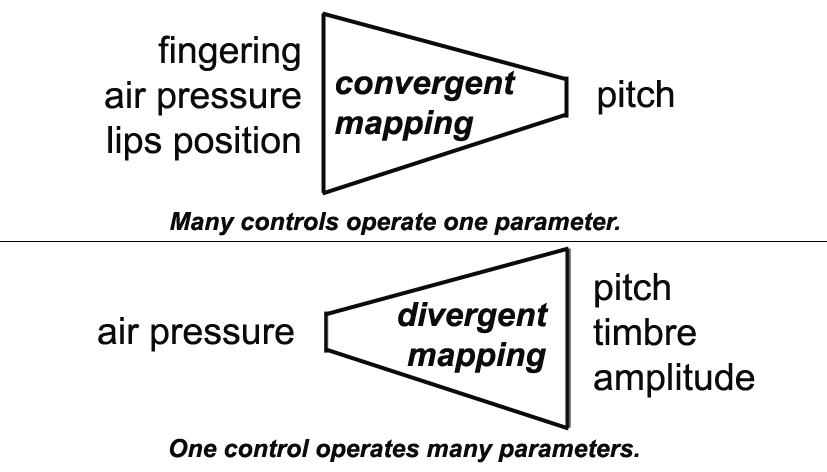
\includegraphics[width=70mm]{CleoPQ-mapping.jpg}}}
\caption{Example of multiparametric mapping of inputs and parameters to control the acoustic flute sound}
\label{Palacio-Quintin:mapping}
\end{figure}

Combinations of convergent and divergent mappings are always experienced while playing an acoustic instrument. It seems much more appropriate to control complex sound processing parameters according to the same principles. These highly non-linear mappings take substantial time to learn, but further practice improves control intimacy and competence of operation.

Different sound processing methods demand different ways of controling them. Mappings must be adapted for each specific situation, and a lot of fine tuning is necessary. I experimented with different combinations of direct, convergent and divergent mapping, some being more suitable to control specific sound processing patches. As my software evolves for each new piece, no definite mapping is possible. However, I try to keep as much consistency as possible in the use of sensors, so that the precision of the control is maintained for each performance. 


\section{Interactive Composition, Improvisation \& Performance}

Joel Chadabe is one of the pionneers of real-time computer music systems. In 1983, he proposed a new method of composition called \emph{interactive composing}, which he defined in the following terms: 

\begin{quotation}
An interactive composing system operates as an intelligent instrument---intelligent in the sense that it responds to a performer in a complex, not entirely predictable way, adding information to what a performer specifies and providing cues to the performer for further actions. The performer, in other words, shares control of the music with information that is automatically generated by the computer, and that information contains unpredictable elements to which the performer reacts while performing. The computer responds to the performer and the performer reacts to the computer, and the music takes its form through that mutually influencial, interactive relationship. \cite[p.144]{Chadabe:1989}
\end{quotation}

From this point of view, the performer also becomes an improviser, structuring his way of playing according to what he hears and feels while interacting with the computer. In most cases, users of interactive computer systems are at once composer, performer and improviser. Due mostly to the novelty of the technology, few experimental hyper-instruments are built by artists. These artists mostly use the instruments themselves. There is no standardized hyper-instrument yet for which a composer could write. It is difficult to draw the line between the composer and the performer while using such systems. The majority of performers using such instruments are concerned with improvisation, as a way of making musical expression as free as possible.  Jonathan Impett also thinks that the use of computers to create real-time music has profoundly changed the traditional kinds of music practices. 

\begin{quotation}
In such a mode of production, the subdivisions of conventional music are folded together: composer, composition, performer, performance, instrument and environment. Subject becomes object, material becomes process. \cite[p.24]{Impett:1998}
\end{quotation}


Using an interactive computer system, the performer has to develop a relation with different types of electroacoustic sound objects and structures. These relationships constitute the fundamentals of musical interaction. The computer part can be supportive, accompanying, antagonistic, alienated, contrasting, responsive, developmental, extended, etc. All the musical structures included in a piece have different roles. Some affect the micro-structure of a musical performance, others affect the macro-structure and many are in between. The interaction between the performer and these musical structures vary. The structures can also support different levels of interactivity between each other. We can divide these structures in 3 distinct types: 

\begin{itemize}
\item sound processing transforming the acoustic sound,
\item sound synthesis,
\item pre-recorded sound material.
\end{itemize}


On the hyper-flute, I have focused on the development of the first type: transforming the flute sound with live digital processing. However, when looking for new extended flute sonorities, the process also leads to the integration of sound synthesis.

In an improvisational context, the interactive computer environment is designed to maximize flexibility in performance. The environnement must give the opportunity to generate, layer and route musical material within a flexible structure, like an open form composition. Ideally, the computer environment would give the same improvisational freedom the performer has developed with his acoustic instrument. Each performer has his personal repertoire of instrumental sounds and playing techniques from which he can choose while performing. This \emph{sound palette} can be very wide, and switching from one type of sound to another is done within milliseconds. Of course, any interactive gestural interface has a limited number of controllers. The sound processing patches can only generate the sounds that have been programmed (even if they include some random processings). The freedom of the performer is somewhat limited by the computer's environment. 

My long term goal is to develop an \emph{interactive sound processing palette} that is as rich and complex as my instrumental one. I want to improvise freely and to be able to trigger many different processes at anytime, and this without disturbing my flute playing. Though there are still programming issues to be addressed before achieving an ideal environment, I have always felt more limited by the number of controllers and buttons on the hyper-flute. This has led me to new developments on the instrument itself.


\section{New Developments}

After eight years of practice, I am now very comfortable playing the hyper-flute. I have also developed a very good knowledge of my musical needs in order to control the live electronics while performing. Over the years, I found what works best and what is missing on the instrument. So I decided to make a new prototype which will feature some new sensors. As I also perform on the bass flute, an hyper-bass-flute is in development. The following sections briefly presents the planned design of those new hyper-instruments.


\subsection{Hyper-Flute}

To maintain the playing expertise I have developed over the years, most sensors used since 1999 will be used in the same physical configuration, but will include technical improvements (ultrasound transmitter, magnetic field sensors on the little fingers, and force sensing resistors under the left hand and thumbs). There will be several more buttons on the new prototype, located close to the right thumb which is more free while playing.

Earlier I mentionned the necessity to have more sensors which do not disturb the hands and fingers while playing. The new prototype is thus designed with a two axis accelerometer placed on the foot-joint of the instrument. This accelerometer gives information about the position of the flute (inclination and tilt of the instrument) in a continuous data stream instead of the simple on/off switches used previously.

The present proprioceptive sensors on the hyper-flute give information about muscle actions that are not visible to the audience (except for the ultrasound sensor and the tilt switches working with the inclination of the instrument). The use of an accelerometer will give more multidimensional data about movements and position which are visible by the auditors. This will help to correlate the amount of activity of the computer with the physical activity of the performer. 

The amount of data produced by the accelerometer greatly increases the possibilities of multiparametric mapping and permits the development of more complex musical structures. This will be very helpful to increase the number of tasks while playing. For example, one can use the inclination to scroll through long menus of different sound processing modules or to choose between several \emph{buffers} to record in. This way, only one button is necessary to trigger many different tasks. As I am already aware of the instrument's inclination while playing (because of the tilt switches), it is now easier to remember the physical position at various angles.

Fastening the sensors on the flute has always been problematic. I own only one (expensive) flute and I do not wish to solder anything onto it. Therefor I have been using double-sided tape to attach the sensors to the flute. This way, the sensors can be taken off when the instrument needs to be cleaned or repaired. But this is a tedious exercise and there is always a risk of breaking them. I am now trying to build the sensors on clips that can easily be attached and removed. This will make it easier to transform any flute into a hyper-flute, and will eventually give opportunities to other performers to play my music.

A first test was to use a \emph{Bo-Pep} for the accelerometer and ultrasound transducer (as showed on Figure~\ref{Palacio-Quintin:bopep}). These plastic hand supports for the flute are simply clipped on the body of the instrument, and can be taken on and off in a second. Some sensors can simply be applied on a \emph{Bo-Pep}, while others will need to use a custom made clip.

% FIGURE 3 Bo-Pep
% [bb=0 0 220 136]
 
\begin{figure}
\centerline{
	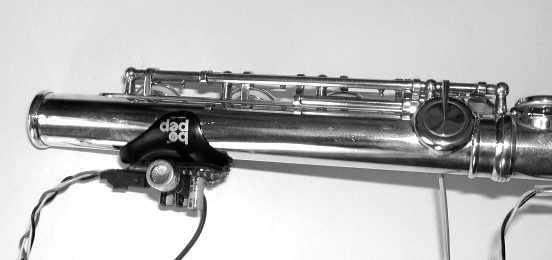
\includegraphics[width=\columnwidth]{CleoPQ-sensors.jpg}}
\caption{Accelerometer and ultrasound transducer mounted on a Bo-Pep}
\label{Palacio-Quintin:bopep}
\end{figure}


\subsection{Hyper-Bass-Flute}

I am also developing a hyper-bass-flute, a noticeably different instrument than the hyper-flute. The bass flute has the advantage of being much bigger so there is more space to attach sensors. Nevertheless, the weight of the instrument limits the capacity of the thumbs to reach different sensors while playing. The new design of the sensors needs to be different than the hyper-flute. Only the accelerometer and ultrasound transducer can be installed on the bass flute as on the flute. Compositional strategies will need to be adapted for this instrument and a new period of learning will be necessary to perform with it. Even if many controllers will be different, I expect the learning process to be much faster due to my experience with the hyper-flute.


\subsection{Interface}

For both hyper-flutes, I will replace the Microlab device with a new interface using the Open Sound Control protocol:

\begin{quotation}
OSC is a protocol for communication among computers, sound synthesizers, and other multimedia devices that is optimized for modern networking technology. Bringing the benefits of modern networking technology to the world of electronic musical instruments, OSC's advantages include interoperability, accuracy, flexibility, and enhanced organization and documentation.This simple yet powerful protocol provides everything needed for real-time control of sound and other media processing while remaining flexible and easy to implement. \cite{Wright:2005} 
\end{quotation}

This protocol will allow the transmission of different types of parameters with more resolution and velocity. This will be achieved with fewer intermediary interfaces and will be much faster. Data will go directly from one interface to the computer through a USB connection. Previously, the Microlab was plugged to a MIDI Interface then to the computer.

A new ultrasonic range finder is being implemented on a PSoC chip by Avrum Holliger at IDMIL. It has a much more refined resolution than the one used on the Microlab, which was limited to 128 values by the MIDI protocol. This new range finder will be directly linked to the main interface.

For the bass flute, it is possible to install the complete interface on the instrument.  The hyper-bass-flute will be connected to the computer with a single USB cable. A prototype is now in development using an Arduino-mini interface which is small enough to fit on the instrument. Wireless connection is not desirable because of its need for power. A 9 volt battery would be too heavy to install on the flute. 

\subsection{Mapping Research Project}

For my doctoral project, my compositions will aim to optimize the mappings of my extended instruments in the context of new computer music pieces. My first intention when building the hyper-flute was to use the natural gestures of the flutist to control sound processing parameters.  However, as stated above, I was obliged to develop new playing techniques to control some of the sensors. 


In the \emph{Performance skills} section, I mention that the ultrasound transducer, pressure sensors and magnet sensors continually capture the natural movement of a performer. It is a  similar situation with the new accelerometer.  Those gestures are directly related to the musical material being performed.

With the new prototype of the hyper-flute, more information from the natural gestures of the performer will be usable. I would like to use these gestures to control the computer so that the performer will not need to add too many extra movements. To achieve this, I will study the gestural data captured by the new hyper-flute (and hyper-bass-flute)~ \cite{Wanderley:2003}.

Instrumental music material will be written first, then performed on the hyper-flutes. The performer will play without taking notice of the sensors. All the gestural data will be recorded together with the flute sound. I will then be able to analyse the gestural data in a specific musical context. This analysis will guide the choice of mappings between the sensors and the computer's live processing parameters. The use of sensors will be precisely specified in a musical context and will be directly related to the performer's natural gestures. This should allow a more subtle and expressive control of the sound processing than is possible in an improvised music context.

To explore the differences of motion between performers, I will record other flutists as well as myself.   I expect other flutists will move more naturally then myself, as I am used to playing with the sensors which react to any movement I make. 



\section{Musical Perspectives}

After 8 years of practice, I consider the hyper-flute as a musical instrument in its own right. New technologies offer opportunities to enhance it but even with these improvements, it will stay the same instrument.  In addition to the development of my improvisational environment, I want to compose more written repertoire. I also hope to have other composers do so as well. My most sincere wish is that eventually other performers will play the hyper-flute. The musical perspectives are open-ended for the hyper-flute, truly a new instrument for the twenty-first century.


\begin{acknowledgement}
I would like to thank Marcelo Wanderley for his invaluable advice in my research and all the IDMIL team for their great technical help. Sincere thanks to Elin S\"{o}derstr\"{o}m and Jean Pich\'{e} for their writing help for this paper. My doctoral studies are supported by the FQRSC (\emph {Fonds qu\'{e}b\'{e}cois de la recherche sur la soci\'{e}t\'{e} et la culture}).
\end{acknowledgement}


\section*{Author Commentary: The Hyper-Flutes, 15 years later}

\paragraph{Cl\'{e}o Palacio-Quintin}

Interest in capturing the gestures of musical performance for interaction with computers has grown extensively in recent decades, alongside quickly-developing technologies that open up many new possibilities. Studies about effective and ancillary gestures, as well as progress in electronics (mainly in the miniaturization of devices) have provided the opportunity to design high-performance hyper-instruments with electronic extensions that are at once more responsive and less intrusive. Many papers published by NIME are documenting this vast research from various point of views.

Nevertheless, there are very few performers who have played consistently on the same augmented instrument for as many years as I have, and there have been almost no publications concerning performance skills on such new instruments. I have been performing with the hyper-flute for 15 years, and it has already been 6 years since I began on the hyper-bass-flute. The instruments themselves have not changed much (the hardware is mainly the same), even if the software developed to play with them evolves with each new work. This long-term dedication to interactive performance on stable interfaces gave me the opportunity to develop a real professional practice. Such a level of virtuosity---like any professional instrumentalist would have on an acoustic instrument---is unfortunately rarely achieved on new interfaces, due both to a lack of dedication over time, and to changes in technology that make interfaces obsolete before even being mastered by any performer. 


% FIGURE 1 - PHOTO 

%\begin{figure}
%\centerline{
%	\includegraphics[width=\columnwidth]{CleoPQ-live_photo_par_Robin_Pineda-2015_BW-small.jpg}}
%\caption{Cl\'{e}o Palacio-Quintin performing \emph{Synesthesia 4: Chlorophylle}. Photograph by Robin Pineda Gould (2015).}			%

%\label{Palacio-Quintin:photo}
%\end{figure}


This article was written in at the beginning of my doctoral research. At that time, I was aiming to expand the repertoire for the hyper-flute and was building the hyper-bass-flute. I achieved these goals and discussed them in my doctoral dissertation~ \cite{Palacio-Quintin:2011}, which presents the compositional processes of six pieces with live interactive electronics that I composed for my hyper-flutes. Each of those compositions attempted to explore different types of musical interactions between the performer and various electroacoustic soundscapes, objects or structures. My last composition \emph{Synesthesia 4: Chlorophylle},\footnote{\url{http://vimeo.com/user2625659}} besides using transformations of the flute sound in real time and granular synthesis from a recorded voice, also included live digital processing of videos and photos, all controlled with the hyper-flute. The use of the performance's gestural data to control these live processing algorithms permitted me to create a work that seems to flow organically. The performer is constantly in dialogue with the electronic parts and contributes to generating them, such that all the elements are interweave to form a whole. Only long term dedication and proximity to the instrument made such seamless integration possible.

As was planned in the Mapping Research Project mentioned in my 2008 article, analysis of the gestural data, captured by the hyper-flute while playing, implied that the composed acoustic flute part preceded and guided mapping choices for the electronics. This analysis, documented in my thesis, has been extremely helpful for optimizing the performer/computer interactions in the work \emph{Synesthesia 4: Chlorophylle}. A summary on this subject was published in Revue Circuit~ \cite{Palacio-Quintin:2012}. I realize now that this work has never been published in English.

In the end, I did not rebuild the hyper-flute entirely, as was planned in 2008, but merely added an accelerometer. I kept using the Microlab interface, which at that time was more powerful and reliable than most smaller new interfaces: (\emph{why change it if it ain't broken!}) The use of the MIDI protocol with that instrument always worked perfectly, and was never a limitation to further software development. The hyper-bass-flute was also designed with a two-axis accelerometer, which gives information about the orientation (inclination and rotation) of the flute. As expected, these accelerometers provide a substantial improvement for gestural capture of movements perceivable by the audience. It also greatly extended the multi-parametric mapping possibilities and helped to correlate the computer's activity with the physical activity of the performer. Now the original prototype of the hyper-flute is aging and is starting to be less reliable. I am planning again to rebuilt it, but will keep most of the design as-is, in order to foster virtuosic practice. 

Over the years, I mainly used Max-MSP/Jitter software for the creation of new works, but recently also started to use Ableton Live in my projects. Ironically, that implies that I now need to reconvert my hyper-bass-flute gestural data into MIDI protocol to interact with the software. In recent years, several composers have written new works for me---Martin Arnold, David Cronkite, Louis Dufort, and Cassandra Miller---but in general, the time available for collaboration was too short for them to fully exploit the possibilities of the hyper-flutes. It is a new instrument and composers, like performers, need time to learn how to use it efficiently. At the time of writing, Monique Jean (Montreal) and Karen Sunabacka (Winnipeg) are composing new pieces for a solo hyper-flutes concert that will be presented across Canada in February 2016. Thus the repertoire for the hyper-flutes is expanding slowly, and my practice keeps evolving, even after 15 years.



\section*{Expert Commentary: Hyper-instruments and Musicianship}

\paragraph{Hans Leeuw}

The first thought that comes to mind when reading the article of Cl\'{e}o Palacio-Quintin about her technical and musical experiences with the hyper-flute is: wouldn't it be a good idea to evaluate all new instruments that come to NIME periodically and systematically? Do they still exist? Are they still used as they were designed? And most importantly: what musical experience is there?
%removed the following footnote (attached to the workd 'hyper-flute' because Cleo already mentions this
%\footnote{The term \textit{hyperinstrument} was coined in 1986 by Tod Machover  at MIT \cite{Machover:1992}} 

I recently interviewed Cl\'{e}o and it is clear that her perspective evolved after having stepped away from her role as instrument designer, to focus on playing the instrument for another seven years. Her story is very interesting for our community. The instrument continues to exist and it is still in development. Not as in ``extra and better sensors,'' but through the experience of the player using the instrument, and composers (including Cl\'{e}o herself) composing for it.

The article makes it clear that Cl\'{e}o's perspective is that of a virtuoso instrumentalist and that her intention is to bring this to the design of the hyper-flute. This is evident, for example, in her mapping choices. These are not aimed at controlling sound syntheses parameters one by one, but rather developed for many-to-many mappings similar to acoustic instruments.

It is also insightful to see that first enthusiasms are not always matched by later process. Cl\'{e}o states that the ``ultrasonic range finder (URF) \ldots turned out to be one of the most useful controllers.'' When interviewed, Cl\'{e}o mentioned that the URF recently broke and now she uses a combination of other sensors to compensate, however she is glad that this afforded new freedom---the URF fixed her position on stage. I had a similar experience with my own instrument: additional electronic valves seemed to be the logical choice when designing my hyper-trumpet \ldots but in fact I rarely use them (though that too might change.)

Such findings can be quite personal and depend on the player's affinity with technology, with music and musical context, and with the musical role the player sees for herself, or simply the professional demands that the player has to deal with---concerts, stipends, commissions, and so on.

It would be interesting to see an article about the experiences with the hyper-bass clarinet SABRe \cite{Schiesser:2012}. This hyper-instrument was developed with the idea of creating a community of players,  and to support sharing of musical experiences. At the moment there are five SABRe's being used. The hyper-flute, the SABRe and my own Electrumpet \cite{Leeuw:2012a} have a common aim of  favouring the achievement of  long term musical development over technological development or the more mundane goal of selling a product.

The above mentioned designers agree on one thing: the musical role of virtuoso performers within the NIME community is valuable and the artistic level of the community can benefit from their input. Christopher Dobrian wrote already in 2006 that the community should ``take advantage of established instrumental skills'' \cite{Dobrian:2006}. That is only one way to put it. There is much more to be learned from real-world players and composers, than just their physical abilities. The next question, in my opinion, is then: ``What does it mean to work professionally with a hyper- (or other semi-digital) instrument?''

Cl\'{e}o's article acknowledges that learning the hyper-flute entailed a long learning process that sometimes contradicted the flute techniques originally learned. She also notices that few performers are willing to put extra time into learning yet another instrument (instead of better learning the one they already play, I would add.)

Even more so, it must be nearly impossible for people who have no musical experience to further develop their instrument after having made an initial design. Such development needs a community of practitioners challenging each other in a competitive manner both as designers and performers. At present the only such community in NIME is the live coding community. However, virtuoso hyper-instrument players can draw from their experience as acoustic players and are often still involved with their instruments in a demanding acoustic environment.

While it is clear that Cl\'{e}o writes from the perspective of an experienced acoustic player with ample experience in the experimental world of electronic music (eight years of playing her hyper-flute), much of the 2008 article is still focused on the link between gestural control and the design of the instrument. It would be very nice to see a new article from her focused on her experience playing her unaltered instrument for seven years (or so) and her musical exchange with other musicians in her field.

